A la hora de estructurar el trabajo que tenemos que hacer en un proyecto de gran magnitud, tenemos que tener en cuenta desde las actividades más ambiciosas hasta las mas detalladas. Por eso, existen diferentes estructuras de datos y formas de organización que nos ayuda a conseguir dicho objetivo. Como bien nos dice el \textit{Atlassian Agile Couch}, para conseguirlo nos podemos servir de los temas, iniciativas, épicas, historias de usuario y tareas. Podemos ver una descomposición visual de estos elementos en la \textbf{Figura \ref{fig:epicasHistorias}}

\begin{figure}[H]
    \centering
    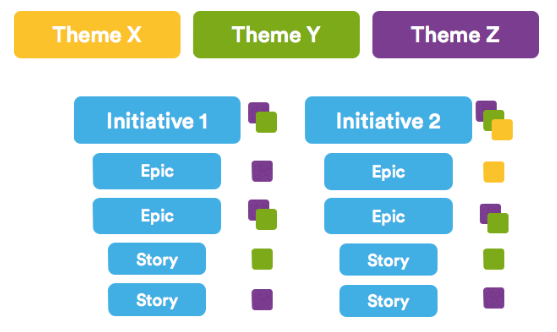
\includegraphics[scale=0.8]{imagenes/diseno/epicasHistorias.png}
    \caption{Relación entre épicas, historias y temas}
    \label{fig:epicasHistorias}
\end{figure}


A modo de resumen, cada una de las estructuras significa:
\begin{itemize}
    \item \textbf{Temas}: son grandes áreas de enfoque que abarcan a toda la organización.
    \item \textbf{Iniciativas}: son conjuntos de épicas que conducen hacia un objetivo común.
    \item \textbf{Épicas}: son grandes cantidades de trabajo que se pueden desglosar en un número de tareas más pequeñas, llamadas historias. 
    \item \textbf{Historias}: son breves requisitos o solicitudes escritas desde el punto de vista del usuario final. 
    \item \textbf{Tareas}: las tareas son actividades que hay que hacer para conseguir desarrollar las historias, no tienen porque estar escritas desde el punto de vista del cliente.  
\end{itemize}

En este proyecto por temas de magnitud, ya que es un proyecto pequeño, solo vamos a contar con historias, tareas y como mucho con unas cuantas épicas que nos van a venir bien a nivel de planificación y explicación del proyecto.

\subsubsection{Épicas}

Las épicas que nosotros vamos a presentar en nuestro proyecto son las siguientes: 
\begin{itemize}
    \item \textbf{Desarrollo}: en esta épica se incluirán las tareas relacionadas con las actividades de desarrollo.
    \item \textbf{Documentación}: se relacionarán tareas de documentación de las diferentes partes que componen el sistema, tanto documentación interna como documentación externa.
    \item \textbf{Configuración}: se añadirán las tareas relacionadas con la configuración de entornos o sistemas necesarios para la consecución de los objetivos del proyecto. 
    \item \textbf{Investigación}: puede que haya algunas tareas de investigación en ciertos puntos del proyecto, en esta épica habrá seguramente muy pocas tareas, pero también considero necesaria añadirla.
\end{itemize}

Cabe destacar que tanto las épicas del proyecto como las diferentes historias de usuario y tareas, las podemos 

\subsubsection{Historias de usuario}

Primero vamos a describir brevemente lo que son las épicas y las historias de usuario. Que son la base de la metodología que estamos siguiendo.

Las historias de usuario son la base trabajo de nuestro equipo de desarrollo. Para presentarlas hemos hecho una pequeña plantilla que muestra las características esenciales de una historia de usuario, y tiene los siguientes campos:
\begin{itemize}
    \item \textbf{Id}: cada una de las historias de usuario de nuestro proyecto va a tener un ID único que la identificará. Esto mejora la búsqueda de las mismas cuando hagamos referencias y siempre sepamos de que elemento estamos hablando. 
    
    \item \textbf{Prioridad Dev.}: número que seguirá la serie de Fibonacci (1, 3, 5, 8, 13, 21) que indicará la prioridad a la hora de desarrollar esa historia de usuario para los desarrolladores. Aclaramos que el 10 será la prioridad máxima y el 1 será la prioridad mínima. 
    
    \item \textbf{Valor}: número que seguirá la serie de Fibonacci (1, 3, 5, 8, 13, 21) que indicará la prioridad a la hora de desarrollar esa historia de usuario para el cliente final. Aclaramos que el 10 será la prioridad máxima y el 1 será la prioridad mínima. 
    
    \item \textbf{Estimación}: una ligera estimación del coste de implementación/finalización de esa Historia de Usuario. Podremos tener diferentes medidas, la mínima serán H (horas) y la máxima serán W (semanas). Ej.: 2H, 3D (días) o 1W. 
    
    \item \textbf{Asignado a}: desarrollador que tendrá asignado esa historia de usuario, aunque las tareas en las que se subdivida puedan estar asociadas a otros desarrolladores. 
    
    \item \textbf{Usuario}: el usuario al que va referida esta historia de usuario dentro de la aplicación final.
    
    \item \textbf{Descripción}: una breve descripción del objetivo que tiene que conseguir esa historia de usuario en concreto.
    
    \item \textbf{Dependencias}: las diferentes historias de usuario de las que depende la historia de usuario especificada. 
    
    \item \textbf{Criterios de aceptación}: los criterios que marcarán cuando la historia de usuario podrá considerarse cerrada y acabada. 
    
    \item \textbf{Épica relacionada}: se mostrará la épica con la que está asociada dicha tarea de usuario. \textcolor{red}{SI TODAS LAS HISOTIRAS VAN A ESTAR RELACIONADS CON UNA EPICA QUE SEA HISTORAS O DESARROLLO DE OALGO ASI, NO TIENE SENTIDO ESTE CAMPO}
    

\end{itemize}

Podemos ver una plantilla del formato que van a tener nuestras historias de usuario en la siguiente \textbf{Figura \ref{fig:formatoHistoria}}

\begin{figure}[H]
\centering
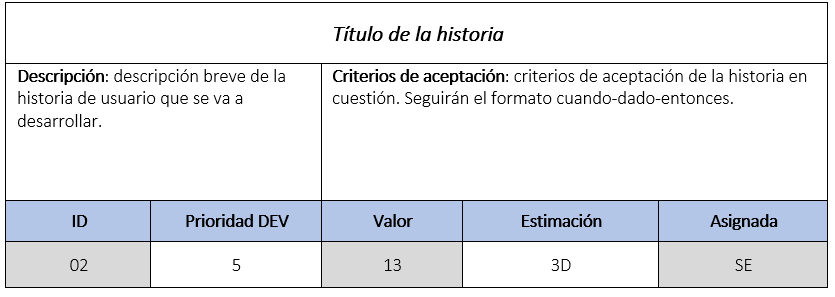
\includegraphics[scale=0.6]{imagenes/diseno/formatoHistoria.png}
\caption{Formato que seguirán las historias de usuario}
\label{fig:formatoHistoria}
\end{figure}

Una vez que hemos definido el formato de nuestras historias de usuario, los criterios que van a tener y todas las partes de las que van a constar, podemos pasar a mostrar todas las que tenemos. 